\section{Introduction}

    Many programs which contain loops or are representing big softwares fall victim to having many redundant code. 
    This could also be possible due to differnt phases of optimization the compiler performs, which leaves certain residual code in each phase.
    One such example of redundant code is that when there are two consecutive reads/writes to the same memory location.
    Another example could be the case that after many optimization passes, certain memory values are not used by the resultant program itself, so the compiler may decide to remove it.
    
    \critic{red}{Consider to give concrete optimization examples here from your notes on optimizations (Clark's lectures).} 

    In a sequential setting the effect of removing such code can be addressed relatively easily as sequential code does not have the complexity of multiple outcomes.
    However, as we saw for instruction reordering, in a concurrent setting, elimination may not be that straightforward. 
    
    Consider the first example in Figure~\ref{elim:example1(a)} below of a Candidate and the resultant candidate after eliminating a write.
    \begin{figure}[H]
        \centering
        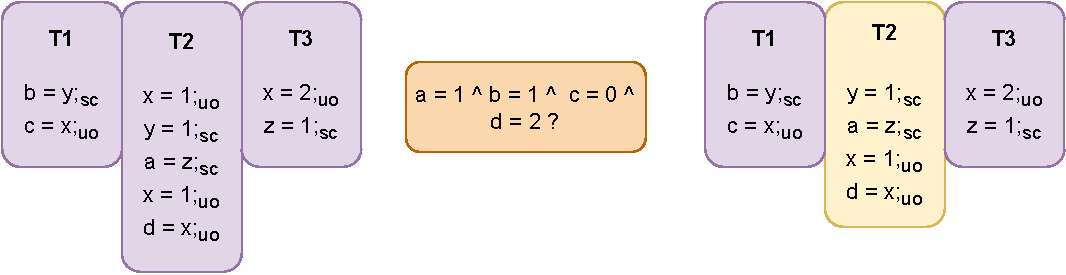
\includegraphics[scale=0.7]{6.Elimination/EliminationExample1(a).pdf}
        \caption{First example for elimination with candidates of the original program and its counterpart after elimination of a write.} 
        \label{elim:example1(a)}
    \end{figure}

    The orange box shows the observable behavior that we want to consider. 
    In the first program, such an outcome should not be allowed. 
    While in the program after eliminating the latter write, this outcome is allowed.
    Figure~\ref{elim:example1(b)} explains the relations formed in a candidate execution that disallow the behavior in question for the original program but justify it after elimination. 
    
    \begin{figure}[H]
        \centering
        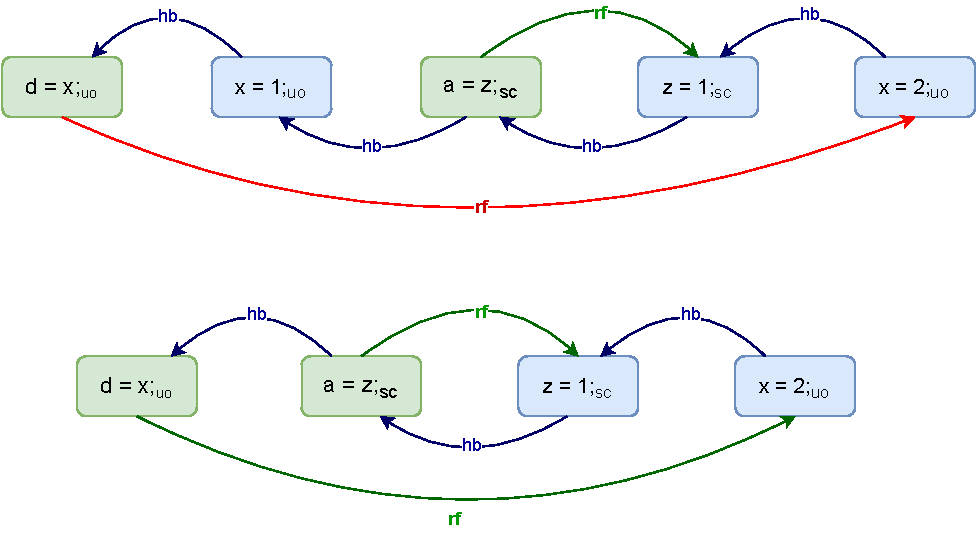
\includegraphics[scale=0.7]{6.Elimination/EliminationExample1(b).pdf}
        \caption{The set of partial order relations justifying the observable behavor in question for both the candidates in Figure~\ref{elim:example1(a)}.} 
        \label{elim:example1(b)}
    \end{figure}

    \critic{red}{Have a better caption for the above figures later. TO better explain them.}

    The first set of relations is for the original program, where Axiom \ref{CoRe} prohibits the read $d$ to have value of $x$ as $2$.
    The second set is for the modified program, where none of the axioms restrict such a behavior (I would suggest the avid readers to check it for themselves).
    
    %For reads
    %I still do not have a counter example to show that elimination of reads is not safe. 
    %This is because I do not yet understand the implications of this on observable behaviors. 
    %Typically, if we remove the read from the set of observables, nothing should change, that is, restrictions on events agent ordered before or after the read must remain as it is.
    %This is because removal of restrictions might lead to new observable behaviors. 
    %The only case where this is not okay is when the read is part of a loop conditional. 
    %Removing such reads from every candidate will resort to non-termination of code.
    %One can jot this down to just restricting elimination of reads that are part of conditionals.
    %But otherwise, one can still eliminate. 
    %I am not sure which other case can be taken. How about showing when two reads are memory ordered without happens-before? Then elimination will not have any use.
    %We can skip this part for now and just refine the previous chapter first.
    In the case of read elimination, we clearly would lose observable behaviors w.r.t. to the read eliminated.
    In addition to this, it becomes difficult to assert whether such an elimination would impact other observable behaviors. 
    For instance, if the reads at the program level represent loop termination checks, then elimination the reads would not be safe as it not only would affect termination, but would also involve elimination of other events at the candidate level.
    